\part{The Web Services}
%% The Web Service is the corner stone of the application. The Web Service is used
%% both to keep weather data up to date, from cron jobs running at external
%% locations, and in addition, to back the front-end of the application.

%% The problem domain investigated in Section~\ref{sec:user_and_task} is the
%% foundation for deriving the resources of the Web Service. After describing the
%% resources and their representations, in Chapter~\ref{chap:resources}, we dig into
%% how to sort out subtleties regarding realizing the data in the resources.

%% Chapter~\ref{chap:gae_ws} and~\ref{chap:ws_daimi} describe the implementation of
%% the Web Service. Because of restrictions in the GAE the Web Service consists of
%% two Web Services: one located at the GAE, and one located at DAIMI. The former
%% chapter describes the implementation of the Web Service at the GAE; and, the
%% latter describes the implementation of the Web Service at DAIMI.

%% While reading this part the reader might wonder where the data in the services
%% will come from. The data in the two Web Services are put in there by Web Service
%% clients described in the next part of the thesis.
\chapter{Resources and their Representations}\label{chap:resources}
Based on the scenarios in Section~\ref{sec:scenarios} we derive the resources for
our Web Service which is the corner stone of the application. The nouns of
the scenarios define the resources in the Web Service: spots, weather stations,
and forecasts. All representations of the resources are in the JSON format.

In the sections about resources we summarize the resources in what we call a
resource view. Together the views describe the resource view of the software
architecture from the resource viewpoint. The concept of views and viewpoints is
presented in \citep{sa:arch_desc}. 
%
\begin{definition}\label{def:resource_viewpoint}
The \emph{resource viewpoint} on the software architecture is concerned with what
resources the system contains and what parts of the uniform interface they expose.
\end{definition}

\section{Spots}
A spot is a geographical point where people wind- and kitesurf. A point is
naturally encoded by latitude and longitude. All spots have a name and
information about its wind directions suitable for surfing; we denote the
property of a spot being apt for surfing (suitable wind in a suitable direction)
as surfability. The directions of surfability are described in a wind
diagram that captures in which directions -- North, North-East, East, etc. -- the
spot is surfable.

Listing~\ref{lst:spotsrep} shows an example of the representation of the spots
resource. The resource is a JSON object that among others contains the following
fields:
\begin{itemize}
  \item \verb|next| is an indicator for \textit{\gls{gls:pagination}}.
  \item \verb|items| a list containing individual spots.
  \item \verb|uri| the URI of the concrete spot.
  \item \verb|forecast_point| the nearest point where forecasts for the spot are calculated for. 
\end{itemize}

The spots resource is the first of three list resources. The list resources have
the same structure: a \verb|next| field which is the URI of the next page or the
empty string if the page is the last and an items field containing the concrete
items. The uniform structure will come in handy when retrieving resources in the
clients.

Spots are connected to the nearest forecast point (soon presented) and the
individual spots, hereby satisfying connectedness.

\begin{lstlisting}[caption=Spots representation, label=lst:spotsrep]
 {
    "next": "",
    "items": [
     {
       "name": "Ahl",
       "country_code": "dk",
       "lat": 56.1729377296,
       "lng": 10.6418412924,
       "wind_diagram": {
	 "S": "YES",
	 "SW": "YES",									
	 "W": "YES",			
	 "NW": "YES"
       },
       "uri": "/spots/ahl/",
       "forecast_point": "/forecasts/56.0,10.5/"
     },
     (...)
   ]
}

\end{lstlisting}
In addition to paging, for performance reasons the list of spots must be subject
to different filters reducing the total number of spots returned; there must
exist filters to reduce the list to
%
\begin{enumerate}
  \item only spots in the proximity of a geographical point; and
  \item only spots in a certain country.
\end{enumerate}
%
The preceding representation is served to the client. We now turn to the
representations sent from the client. 

Spots are created by any user in the system. The application receives concrete
spot resource representations to either create or update spot resources.  The
representation of spots accepted from the client at the server is different than
those sent to the client. The representations accepted from the client are in the
format that browsers submit data in: the official name is
\verb|application/x-www-form-urlencoded| \citep[sec.17]{w3:HTML}, we denote it
uri-encoding from now on. The difference in format is because we rely on Django
forms on the server side. Django forms gives much for free, including validation
of fields, error messages to return to the user, and acceptance of
uri-encoded data directly. A uri-encoded spot representation looks like the
following:
\begin{verbatim}
name=Ahl&lat=56.172&lon=10.641&country_code=dk&S=YES
\end{verbatim}

\begin{table}[htbp]
\centering
\setlength\extrarowheight{3pt}
\begin{tabularx}{\textwidth}{l X}
\toprule
Resource URI    & Action\\\midrule
\verb|/spots/|  
                & \verb|GET| all spots at page 1\\
\verb|/spots/{country_code}/|
                & \verb|GET| all spots in a certain country\\
\verb|/spots/|  
                & \verb|POST| a new spot\\
\verb|/spots/{spot name}/|
                & \verb|PUT| a new representation of an existing spot\\
\verb|/spots/{spot name}/|
                & \verb|DELETE| an existing spot\\
\bottomrule
\end{tabularx}
\caption{Resource view of spot resources}\label{tab:spot_resources}
\end{table}
An overview from the resource viewpoint of the resources discussed in this
section is given in Table~\ref{tab:spot_resources}. The URIs support the naming
conventions stated in \citep[p.117-118]{rest:webservice}; this means,
\begin{itemize}
 \item \verb|/| indicates a \verb|parent/child| resource hierarchy;
 \item \verb|,| or \verb|;| indicate no hierarchy. The former indicates that the
 order is significant, e.g., the latitude and longitude pair \verb|56.0,10.5|,
 whereas the latter indicate that the order is insignificant. Inputs that
 conceptually are arguments to an algorithm are indicated with query parameters.
\end{itemize}

\section{Weather Stations}\label{sec:res_weather_stations}
A weather station is a place where observations are created. Observations
consist of a time, a wind velocity measurement, and a temperature
measurement. The application currently has three resources for live weather data
DCA, DMI, and WB.

\subsection*{DCA and DMI}
Live weather data -- wind speed and gust, temperature, and direction measurements
-- are available at DCA (of the west coast in Jutland) and DMI (most regions in
Denmark). 

The latest observation is interesting and is exposed as a resource. In addition,
it is relevant to know whether the wind picks up or slacks down based on the last
observations. Therefore a list of weather observations belonging to a specific
station is a resource. The latest observations is incorporated into the weather
stations resource; the reason is that the last observation is needed in most
cases, and this is not the case for the rest of the observations.

Listing~\ref{lst:weather_stations} shows an example of the representation of
weather stations. The resource is a JSON object that among others contains the
following fields:

\begin{itemize}
  \item In the JSON list, \verb|items|, the \verb|uri_extern| field specifies the
URI of the weather station at the external location: the external page to link
to. The page to scrape is identified by \verb|uri_scrape|.
  \item The last two fields in the list are links to the weather station and its
  observations respectively, thereby satisfying the constraint of connectedness.
  \item The timezone field is used to convert the UTC observation time stored in
  the database to the time where the weather station is located when JavaScript
  is not available.
\end{itemize}

\begin{lstlisting}[caption=Weather stations representation, label=lst:weather_stations]
{
  "next": "/api/weather_stations/?geohash_offset=swgv3sxf003p"}  
  "items": [
    {
      "name": "Skagen", 
      "lat": 57.723952722299998, 
      "lon": 10.5997467041016, 
      "timezone": "Europe/Copenhagen", 
      "type": "DCAWeatherStation", 
      "latest": {
        "direction": 242.90000000000001, 
        "icon": "/images/wind_arrows/SW_4to6.png", 
        "speed": 5.9000000000000004, 
        "temp": 13.0, 
        "time": "2009-06-19T12:00:00"}
      },
      "uri": "/api/weather_stations/dk/skagen/",
      "uri_extern": "http://www.kyst.dk/sw3029.asp", 
      "uri_observations": "/api/weather_stations/dk/skagen/observations/", 
      "uri_scrape": "http://www.kyst.dk/custom_asp/defaultjs.asp?id=3003&targetStation=1100"
    },(...)
  ]
}
\end{lstlisting}

The representation for observations for a specific resource is a list of objects
containing weather data; an example is shown in Listing~\ref{lst:obs_res}. The
\verb|time| field indicates the time of the observation in UTC time, the
\verb|speed| and \verb|gust| field indicates the speed in \verb|m/s|, the
\verb|direction| field is the direction in degrees where the wind is blowing
from, and the \verb|icon| field is a link to a representative direction and speed
icon. 

\begin{lstlisting}[label=lst:obs_res,caption=Observations representation]
{
  "owner": "/weather_stations/dk/skagen/",
  "page": 1,
  "has_next": true,
  "items": [
    {
      "direction": 242.9, 
      "icon": "/images/wind_arrows/SW_4to6.png", 
      "speed": 5.9, 
      "temp": 13.0, 
      "time": "2009-06-19T12:00:00"
    },
    (...)
    ]
}
\end{lstlisting}

\subsection*{WeatherBug}
DCA and DMI produce weather observations only for Denmark; additional resources
are needed.

WeatherBug provides an API to access weather information worldwide. We use the following
functions from the API:
\begin{itemize}
  \item retrieve an XML list of stations in the proximity of a latitude and longitude; and,
  \item retrieve an RSS feed of live weather data for a specific weather station.  
\end{itemize}
Representations of the weather resources are obviously already created. The
existing representations, at first sight, open the option to completely bypass
the application server and let JavaScript retrieve the relevant weather data
directly from WeatherBug. The representations, however, are not in JavaScript
format which makes it impossible to load data directly into browser
clients because of the same origin policy described in Section~\ref{sec:json}.

Another option is storing the data on the GAE server and update the content as it
becomes stale. This approach is the only option that serves data fast enough and
is therefore chosen. Following the approach weather stations are subject to
frequent updates of observations. Updates are uploaded from a Web Scraper located
at an external machine. We expose the \verb|POST| method of the observations
resource to post observations to since the concrete URI of the posted resource is
unknown. The observation representation accepted from the client is in JSON
format, and is just a single item of the observations list shown in
Listing~\ref{lst:obs_res}. 

We use the same representation for WeatherBug stations as for DCA and DMI weather
stations. An overview of the resources is given in Table~\ref{tab:ws_resources}. 

\begin{table}[htbp]
\centering
\setlength\extrarowheight{3pt}
\begin{tabularx}{\textwidth}{l X}
\toprule
Resource URI    & Action\\\midrule
\verb|/weather_stations/|  
                 & \verb|GET| all weather stations\\
\verb|/weather_stations/{country_code}/|
                 & \verb|GET| all weather stations in a certain country\\
\verb|/weather_stations/{id}/observations/|
                 & \verb|GET| all weather observations\\
\verb|/weather_stations/{id}/observations/|
                 & \verb|POST| a new weather observation\\
\bottomrule
\end{tabularx}
\caption{Resource view of weather station resources}\label{tab:ws_resources}
\end{table}

\section{Forecast Points}\label{sec:res:forecast_points}
A forecast point is a specific point on the Earth where forecasts are calculated
for. A forecast is a prediction of the weather at some specific time for a
specific forecast point.

A natural source for forecasts is DMI; however, their forecast data is
unavailable and they have no interest in joining in on a collaborative
project. The National Oceanic Atmospheric
Administration\footnote{\url{http://www.noaa.org/}} (NOAA) in the US, however, by
law puts weather data into the public
domain\footnote{\url{http://www.weather.gov/disclaimer.php}}. This means use of
their data is allowed in almost any context, and that we can be certain that the
service continues.

NOAA produces many highly detailed forecast for the US, and in addition global
forecasts using the Global Forecast System\footnote{Info about the GFS model
\url{http://www.emc.ncep.noaa.gov/modelinfo/index.html}} (GFS). The forecasts are
made four times daily at 00, 06, 12 and at 18 o'clock UTC. At these four times
detailed forecasts are calculated for the next 48 hours with a three hour
interval between them; actually there are forecast with a longer prediction in
the future but these are of decreasing detail. The most detailed GFS forecasts
produced at NOAA are produced at a degree of 0.5�.

A note on accuracy: the earth has latitudes in the interval [-90�;90�]. This
gives a total of 360 points along \textit{\gls{gls:meridian}}s that are subject
for forecasts. Longitudes are values in the interval [-180�;180�]. This yields
720 points. Looking at a map we can see that in this resolution, e.g., Aarhus and
Skanderborg probably are associated with the same grid location.

Detailed NOAA GFS forecasts are located at
\url{http://nomad3.ncep.noaa.gov/pub/gfs/rotating-0.5/}. In the directory there
are three important types of files:
%
\begin{enumerate}
  \item Forecasts in GRIB2 format named \verb|gfs.t{TT}z.pgrb2f{XX}|;
  \item inventories for forecasts named \verb|gfs.t{TT}z.pgrb2f{XX}.inv|; and
  \item descriptor files for a specific run named \verb|gfs_t{TT}z.ctl|; 
\end{enumerate}
% 
In the above \verb|TT| is the time of the calculation and \verb|XX| is a delta in
hours to add to the time of calculation to get the time of the prediction. In the
descriptor file all the fields in the forecasts are defined. For now we are
interested in the wind forecast which is given by a vector split up into a \verb|u| and a
\verb|v| component of the wind 10 meters above the ground. In addition, we are
interested in the temperature forecast near the surface given by a single field
where the value is reported using the Kelvin scale. The value of the fields is
retrieved by, e.g., \verb|wgrib2| introduced in Chapter~\ref{chap:forecasts}.

\begin{lstlisting}[caption=Forecast points representation, label=lst:forecast]
{
  "next": "",
  "items": [{
      "lat": 36.5, 
      "calculation_time": "2009-07-01T06:00:00", 
      "lon": 29.0,
      "uri": "/api/forecast_points/36.5,29.0/", 
      "forecasts": [{
          "direction":252.53999999999999, 
          "icon": "/images/wind_arrows/W_6to8.png",
          "speed":6.5300000000000002, 
          "temp": 27.050000000000001, 
          "time": "2009-07-01T12:00:00"},
        (...)
      }
    (...)
  ]
}

\end{lstlisting}

Listing~\ref{lst:forecast} shows the representation of forecasts for a specific
point. It contains the time of forecast calculation, and the forecasts. An
overview of the resources is given in Table~\ref{tab:for_resources}.
\begin{table}[htbp]
\centering
\setlength\extrarowheight{3pt}
\begin{tabularx}{\textwidth}{X X}
\toprule
Resource URI    & Action\\\midrule
\verb|/forecast_points/|  
                & \verb|GET| all points\\
\verb|/forecast_points/{lat},{lon}/|
                & \verb|GET| a forecast point representation\\
\verb|/forecast_points/{lat},{lon}/|
                & \verb|PUT| a new forecast point representation\\
\bottomrule
\end{tabularx}
\caption{Resource view of the forecast points resources}\label{tab:for_resources}
\end{table}
Updates of a point's forecasts are supported by exposing the \verb|PUT| method of
the uniform interface. The representation accepted is in the same JSON format.

In comparison to weather station resources, forecast point resources have no
weather data resources belonging to it. Forecast point resources consist of both
forecast point information and all the forecasts. The reason for deviating is
that all weather data of the forecast point belong to a specific calculation time
of the forecast point making it more natural to think of all the content as a
single resource.

\section{Sorting out the resource requirements}\label{sec:proximity}
In the last section we pointed out the resources in the Web Service, not how to
process the content in them. Filtering points on a proximity basis is
non-trivial. This section reviews our solution.  

The application will eventually contain a huge data set: spots, weather stations,
forecast points, etc. Returning the whole data set is infeasible in terms of
latency at the client.  In addition, we have a
\textit{\gls{gls:location_based_service}} requirement. To sum up, filtering by
location reduces the data set, and increases the relevancy of the data
set. Therefore, the application needs a filter on points which returns a subset
of points in the proximity of a certain place.

Filtering on proximity sounds like a rather easy problem but it is not. To limit
the result set, in a usual database several inequality filters are applied to the
latitude and longitude values creating a bounding box. As mentioned in
Section~\ref{sec:queries}, the datastore can only apply inequality filters on a
single property; a bounding box demands two: an index on latitude and an index on
longitude. Listing~\ref{lst:proximity_query} shows a dysfunctional GAE query that
one could think would solve the problem.

\begin{lstlisting}[label=lst:proximity_query,caption=Dysfunctional GAE bounding box query]
>>> from wlw.models import Spot
>>> from google.appengine.ext import db
>>>
>>> point_1 = db.GeoPt(lat=50, lon=-10)
>>> point_2 = db.GeoPt(lat=60, lon=0)
>>> q = db.Query(Spot) \
...   .filter('point >', point_1) \
...   .filter('point <', point_2)
>>> for s in q:
...    print 'spot: %s \npoint: (%s)' % (s.key().name(), s.point)
...
spot: ahl
point: (56.1729377296,10.6418412924)
\end{lstlisting}

The filters in the query apparently set up a bounding box, but, because of the
inequality filter restriction the query ignores the longitude boundary given by
the \verb|GeoPt| property, and only filters on the latitude. The problem results
in GAE returning \textit{all} spots that lie within the given latitudes, in this
case only one: Ahl.

We present two approaches to the problem, where the first is an obvious solution,
but it does not scale as the data set gets large. The other, is a scalable
solution based on geohash.

\subsection{Calculating proximity points with haversine}
Finding proximity points is possible by first calculating the distance between a
reference point and all other points; afterwards, filtering out points over a
certain threshold distance to the reference point.

In the following we assume the Earth is a sphere ignoring the fact that best
approximation is an oblate spheroid\footnote{http://en.wikipedia.org/wiki/Earth}.

%
A great circle is a circle on a sphere which cuts the sphere into two equally
sized halves, i.e, the circle has radius equal to the radius of the sphere and
the same center as the sphere. An area on the sphere bounded by three arcs of
great circles that do not all have a common point is called a spherical
triangle. The (shortest) distance between two points on a great circle is the
shortest possible distance between the two points, since the arc on the great
circle is the arc with the smallest deviation from a straight line.  Looking at
Figure 5.1, which shows a spherical triangle, the arc c along the great circle is
the shortest distance between A and B. 
%
\begin{figure}[htbp]
  \centering
  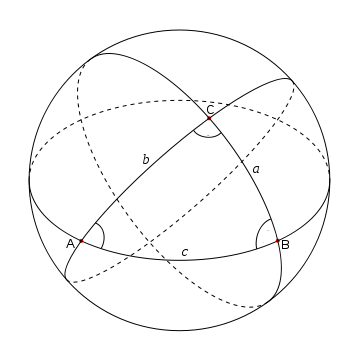
\includegraphics[width=8cm]{./Figures/spherical-triangle2}
  \caption{Illustration of a spherical triangle}
  \label{fig:spherical_triangle}
\end{figure}
In a spherical triangle in a unit sphere the law of cosines relates the sides and
angles of the triangle, in the following way:
%
\begin{theorem}\label{thm:law_of_cosines}
Spherical law of cosines \citep[p.130]{mat3}
\begin{equation}
  cos(c) = cos(a)cos(b) + sin(a)sin(b)cos(C) 
\end{equation}
\end{theorem}
%
Isolating $c$ in the formula gives the distance between the points $A$ and
$B$. However, when $c$ (the distance) is small rounding errors are stated to be
significant \citep{gis:haversine,wiki:haversine,haversine:sinnott}, therefore,
instead the haversine formula is used \citep{haversine:sinnott}. The formula is
based on the haversin function, defined as:
%
\begin{equation}
  haversin(\theta) = sin^2(\frac{\theta}{2})
\end{equation}
%
The following identity between $cos$ and $haversin$ exists:
%
\begin{align}
  cos(2\theta) &= 1 - 2sin^2(\theta) \notag\\
  \tag{double-angle formula \citep[p.A23]{math:stewart}}\\
  cos(\theta) &= 1 - 2sin^2(\frac{\theta}{2}) = 1 - 2haversin(\theta) \label{eq:rel_cos_hav}
\end{align}
%
We now derive the law of haversines from the spherical law of
cosines. Substituting $cos$ with $haversin$ using (\ref{eq:rel_cos_hav}) in the law
of cosines, we get:
%
\begin{align}
  1 - 2haversin(c) &= cos(a)cos(b) + sin(a)sin(b)(1 - 2haversin(C))  \notag\\
  1 - 2haversin(c) &= cos(a-b) - 2sin(a)sin(b)haversin(C) \notag\\% cos(a-b) substitue with haversine \\
  \tag{Using the subtraction formulas \citep[p.A23]{math:stewart}}\\
  1 - 2haversin(c) &= 1 - 2haversin(a-b) - 2sin(a)sin(b)haversin(C) \notag\\
  \tag{Substituting $cos$ with $haversin$}\\
  2haversin(c) &= 2haversin(a-b) + 2sin(a)sin(b)haversin(C) \notag\\
\end{align}

\begin{theorem}
The law of haversines
\begin{equation}
    haversin(c) = haversin(a-b) + sin(a)sin(b)haversin(C) \notag
\end{equation}  
\end{theorem}
%
We note that $a$, $b$, and $c$ given in radians are equal to the length of the
arcs, since we are working on a unit sphere. Now let $C$ be placed on the North
Pole, then by definition its latitude is 90� or in radians $\frac{\pi}{2}$. Then,
the length of the arcs $a$ and $b$ are:
\begin{align}
  a &= \frac{\pi}{2} - B_{lat} \notag\\
  b &= \frac{\pi}{2} - A_{lat} \notag
\end{align}

%
Let $\Delta lat$ and $\Delta lon$ be the latitude and longitude differences between
$A$ and $B$ respectively, then since,
\begin{equation}
  sin(\phi) = cos(\frac{\pi}{2} - \phi) \label{eq:sin_cos}
\end{equation}
we have
\begin{equation}
  haversin(c) = haversin(\Delta lat) + cos(a_{lat}) * cos(b_{lat}) * haversin(\Delta lon)
\end{equation}
%
In the general case for a sphere with arbitrary radius the unit circle distance
$c$ is related to the real distance $d$ on the sphere by: $c = \frac{d}{radius}$  
%
\begin{theorem}
The haversine formula
\begin{equation}
  haversin(\frac{d}{radius}) = haversin(a_{lat}-b_{lat}) + cos(a_{lat}) * cos(b_{lat}) * haversin(b_{lon}-a_{lon}) \notag
\end{equation}
\end{theorem}
%
By isolating $d$ the distance is found:
\begin{equation}
sin(\frac{d}{2R}) = \pm \sqrt{haversin(\Delta lat) + cos(a_{lat}) * cos(b_{lat}) * haversin(\Delta lon)} \label{eq:dis1}
\end{equation}
\begin{equation}
sin(\frac{d}{2R}) = \sqrt{haversin(\Delta lat) + cos(a_{lat}) * cos(b_{lat}) * haversin(\Delta lon)} \label{eq:dis2}
\end{equation}
\begin{equation}
\frac{d}{2R} = arcsin(\sqrt{haversin(\Delta lat) + cos(a_{lat}) * cos(b_{lat}) * haversin(\Delta lon)}) \label{eq:dis3}
\end{equation}
\begin{equation}
d = 2R*arcsin(\sqrt{haversin(\Delta lat) + cos(a_{lat}) * cos(b_{lat}) * haversin(\Delta lon)}) \tag{the distance formula}  
\end{equation}
\\\\ In~(\ref{eq:dis3}) $arcsin$ returns the value of $\frac{d}{2R}$ in the
interval $[0,\frac{\pi}{2}]$. There is also a solution to (\ref{eq:dis2}) in
$[\frac{\pi}{2},\pi]$ but this solution is not relevant since we are interested
in the value of $\frac{d}{R}$ in $[0,\pi]$.

\subsubsection{Distance formula in Python}
The distance formula is easily implemented in Python, shown in
Listing~\ref{lst:haversine}. An example of calculating the distance between two
points is shown in Listing~\ref{lst:haversin_applied}.
\begin{samepage}
\begin{lstlisting}[caption=Python implementation of distance calculation using the haversine formula,label=lst:haversine]
from math import sin, atan2, cos, sqrt, pi

earth_radius = 6371
radian = pi / 180

def distance(point1, point2):
    '''Calculates the distance between two points, using the haversine formula.
    '''
    lat_a, lon_a = to_radians(point1)
    lat_b, lon_b = to_radians(point2)
    dlon = lon_b - lon_a
    dlat = lat_b - lat_a

    haversin_c = (sin(dlat/2))**2 + cos(lat_a) * cos(lat_b) * (sin(dlon/2))**2 

    # unit sphere distance
    c = 2 * asin(sqrt(haversin_c)) 

    distance = earth_radius * c
    return distance

def to_radians(point):
    '''Convert to radians.
    '''
    lat = point.lat * radian
    lon = point.lon * radian
    return lat, lon
\end{lstlisting}
\end{samepage}

\begin{samepage}
\begin{lstlisting}[caption=Calculating the distance between Aarhus and Aalborg,label=lst:haversin_applied]
>>> import geo,math
>>> class Point:
...     def __init__(self,lat,lon):
...             self.lat = lat
...             self.lon = lon
...
>>> aarhus = Point(56,10)
>>> aalborg = Point(57, 10)
>>> geo.distance(aarhus, aalborg)
111.12511347447912
\end{lstlisting}
\end{samepage}

\subsubsection{Why haversine? A small experiment}
We derived haversine based on the statements that using the spherical cosines
relation to calculate distance would cause significant rounding errors with small
distances. What is small in a modern context? In order to reason about this we
have implemented the direct approach to the distance calculation as well and
compared it with distance calculation based on the haversine formula.

\begin{table}
\centering
\begin{tabularx}{\textwidth}{l l l l l}
\toprule
Point       & Point                & Haversine Distance (m)& Cosines Distance (m) \\\midrule
(56.0,10.0) & (57.0,10.0)          & 111125.113474    & 111125.113474   \\
(56.0,10.0) & (56.0000009537,10.0) & 0.105977166514   & 0.0948756933212 \\
(56.0,10.0) & (56.0000004768,10.0) & 0.0529885829037  & 0.0             \\
\bottomrule
\end{tabularx}
\caption{Comparing distances calculated with haversine and cosines}
\label{tab:hav_cos_comp}
\end{table}

Table~\ref{tab:hav_cos_comp} summarizes the results using Python on a 32-bit
machine. There is a maximum difference of 5 cm between the two approaches. We
conclude that the reasoning for the haversine formula is irrelevant in a modern
context for most distance calculations on the Earth. Since we have derived
haversine we continue using it. The reader can refer to
Appendix~\ref{AppendixHaversine} for the implementations and the whole transcript
of the output of the experiment.

\subsubsection{Sorting by distance}
Sorting points by distance is easy exploiting the haversine function, as shown in
Listing~\ref{lst:haversine_sort}. Python's included \verb|sort| function can sort
using any comparator. In this case the comparator calculates the distance, using
the distance formula, between the current point and the reference point.

\begin{lstlisting}[label=lst:haversine_sort, caption=Sorting points with haversine]
def sort_by_distance(ref_point, entities):
    '''Sort entities with a point property, by distance wrt. a reference point.
    
    Args:
        entities: list of entities with a point property.
        ref_point: reference point to calculate distance from.
    Returns:
        list of entities sorted by distance. The distance is added as a member of the entity. 
    '''
    def _distance_to(entity):
        d = distance(ref_point, entity.point)
        entity.distance = d
        return d
    
    entities.sort(key=_distance_to)
    return entities
\end{lstlisting}

There is a problem with the approach using the haversine formula; it is
impossible to calculate an index in the Google datastore to support the distance
formula. Therefore finding spots within a certain distance involves a full table
scan, iterating over all spots in the database, and for each spot calculating the
distance to the reference point. 

Haversine is useful for calculating the distance between few points, but
increasing the number of points demands another approach that reduces the data
set and exploits indexing and preserves scalability. In the next section, we
present an alternative approach.

\subsubsection{Calculating proximity points with Geohash}
Geohash, invented by Gustavo Niemeyer, is an algorithm to convert between
latitude and longitude coordinates and a hash value \citep{wiki:geohash}. In
essence, geohash is just a z-order space-filling curve. Therefore a database can
benefit from a usual index on geohashed points when performing searches for
points in the proximity of each other.

Geohash is based on a custom \textit{\gls{gls:base_32}} alphabet for encoding and
decoding binary data. The custom alphabet is given by the string
\verb|"0123456789bcdefghjkmnpqrstuvwxyz"|. The index of a character in the string
is equal to the value of the character, e.g., 'z' has the associated value 31
which is $11111_2$.

Geohash supports arbitrary precision in the encoding of geographical points by
interleaving the latitude and the longitude in the bit string. A bit string such
as $b = 11111$ is decoded to a latitude longitude point as follows:

\begin{itemize}
\item Even positioned bits pertain to longitude:
\begin{math}
b_{lon} = b_0b_2b_4 = 111
\end{math}

\item Odd positioned bits pertain to latitude:
\begin{math}
b_{lat} = b_1b_3 = 11
\end{math}
\end{itemize}

\begin{figure}[htbp]
  \centering
  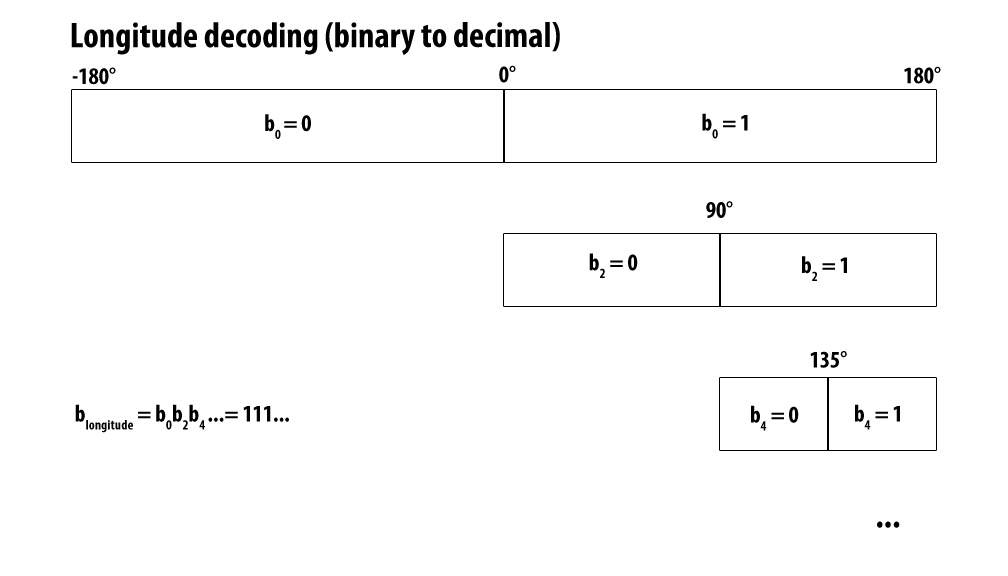
\includegraphics[scale=0.3]{./Figures/geohash_decoding_lon}
  \caption{Geohash longitude calculation}
  \label{fig:geohash_calc}
\end{figure}

Every bit in $b_{lon}$ and $b_{lat}$ halves the point's location space. When the
bit is set the upper half is chosen. The longitude of geohash 'z' is therefore
between [135�,180�], as shown in Figure~\ref{fig:geohash_calc}, and the latitude
is between [45�,90�]. All points with prefix 'z' are in this area. A specific
point is calculated by taking the mean value of the range; thus, the geohash 'z'
equals the point (67.5�, 157.5�).

There are two Python geohash implementations available: \citep{geohash:erle}
which is in the public domain and \citep{geohash:norrgard} which is licensed
under GNU Affero General Public License (AGPL)\footnote{AGPL is a somewhat more
restrictive license than GPL. A Web application based on GPL software must only
open source the software if the software running the service is distributed to
others. AGPL, in essence, demands that the software running the Web application
is open sourced also if the software is not distributed.}. The former is a bit
more advanced; it supports addition of geohashes, and has two formats for the
hash: binary and character based. The result of an addition is the minimal
bounding box of the two geohashes. An example of the usage of the first
implementation is shown in Listing~\ref{lst:geohash_example}. Note that the usual
convention of the sequence latitude and longitude is reversed to longitude and
latitude. The last line in the example shows that the implementation is buggy
when decoding hashes. We have just shown above that the point represented by 'z'
was (67.5�, 157.5�) and this is not the case here, the longitude is wrong. On the
server in the application we encode geographical points using
\citep{geohash:norrgard}.

\begin{lstlisting}[caption=Geohash example usage,label=lst:geohash_example]
>>> import geohash
>>> london_west = geohash.Geohash((-0.12,51.50))
>>> str(london_west)
'gcpuvr295zcd2'
>>> london_east = geohash.Geohash((0.12, 51.50))
>>> str(london_east)
'u10hfxr3hpy6q'
>>> world = london_east + london_west
>>> str(world)
''
>>> geohash.Geohash('z').point()
(180.0, 67.5)
\end{lstlisting}
%
Listing~\ref{lst:geohash_example} also shows a general problem with geohasing: the
property of similar prefixes of points in the proximity of each other is not
always true. The problem lies within proximity points with different prefix. Take for
instance the area just West of London, Greenwich; the hash of the western side
(bit 0 unset), has a complete different prefix than the hash of the eastern side
of Greenwich (bit 0 set) because boxes have a borderline here: namely the prime
meridian. Restricting proximity points to a certain prefix results in lost
proximity points.

\subsubsection{Lost proximity points: a solution}\label{sec:lost}
The \gls{gls:base_32} alphabet and the algorithm of geohash result in a
conceptual grid that is overlayed on the Earth, shown in
Figure~\ref{fig:geohash}. This grid is essential in solving the problem of lost
proximity points.

\begin{figure}[htbp]
  \centering
  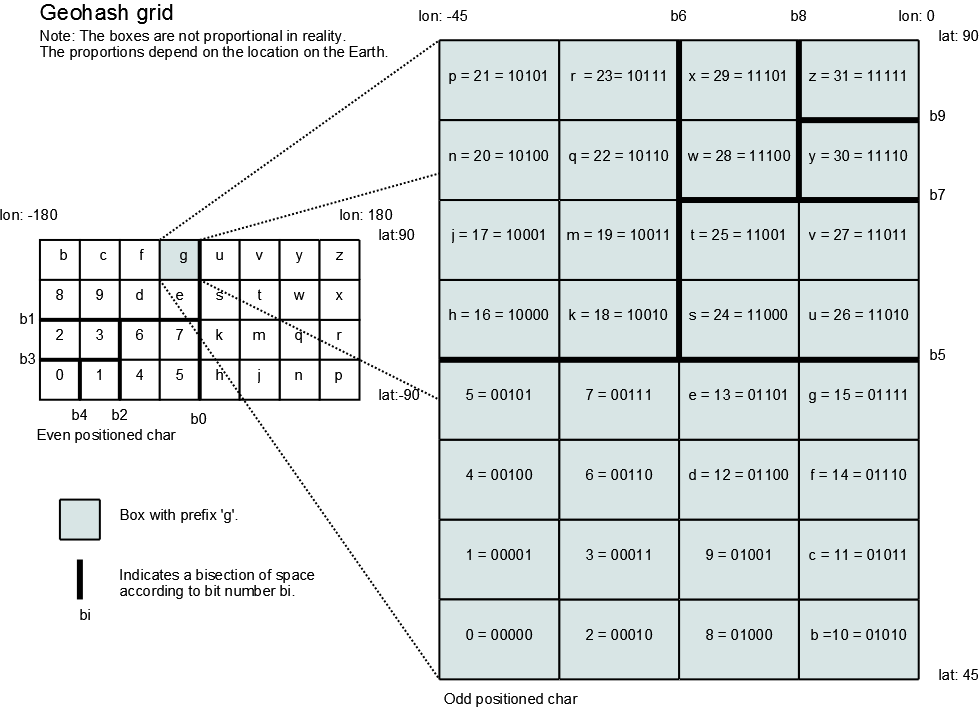
\includegraphics[scale=0.3]{./Figures/geohash}
  \caption{Cylindrical projection of Geohash grid}
  \label{fig:geohash}
\end{figure}

A solution to the proximity problem is augmenting the returned data set with
points from all the grid boxes surrounding the requested one: the neighbors
directly to the north, northeast, east, etc.

The geohash grid has a recursive structure: every char in a geohash specifies a
grid box container, and the next char in the geohash specifies a grid box within
the first grid box container, and so on. The position of the char, even or odd,
decides which of the two containers in the figure is representative for the char,
since even positioned chars begin with an even bit, and odd positioned chars
begin with an odd bit.

We have implemented a solution where the two representative grids are represented
as matrices: allowing for easy navigation to the neighbors of a grid
box. Navigating to neighbors falls into three cases:

\begin{enumerate}
  \item the neighbor is in the same container; 
  \item the neighbor is in a neighbor container; or,
  \item the neighbor is on the other side of the cylindrical projection, i.e.,
  crossing the ends of the square cylindrical projection.
\end{enumerate}
%
Locating a neighbor in the first case is easy: for all neighbors return their
geohash, which is the current geohash with the last char replaced by the char
representing the new location in the container.

Locating the neighbors in the second case is more tricky. The case is identified
by going out of bounds of the matrix. By wrapping around the indexes we identify
the new suffix of the grid box we are after, i.e., if the request is for the
Eastern neighbor of geohash 'z' the index is wrapped around to the other side
which is 'b' (in the even case). However, as we are out of bounds, we need to
zoom out and still find the eastern neighbor. Zooming out and tracking the
neighbor is equal to doing the same query on the geohash with the last char
stripped.

If the container of 'z' has an eastern neighbor the tracking succeeds and we can
return the char of the eastern container concatenated with the suffix identifying
the grid box within it, found when wrapping around. 

The third case happens when we are fully zoomed out: in this case there exist no
neighbors in the grid; however, the logical neighbor is still found by wrapping
around (this only makes sense for East-West directions). We can think of this as
connecting the ends of a square map of the world assuming it is created by a
cylindrical projection.

An excerpt of the implementation of geohash neighbors is shown in
Listing~\ref{lst:geohash_neighbor}. The main method is \verb|step_in_direction|
which returns the grid box, at the same zoom level, which is the neighbor to the
box of the given geohash in the requested direction. The function calls itself
recursively when it must zoom out to find the neighbor. Under the recursive call
it keeps the found suffix of the neighbor in the \verb|new_geohash_suffix|
argument, and when a neighbor is found the char of its grid box is concatenated
with the \verb|new_geohash_suffix| resulting in another geohash suffix. At last
the suffix if prefixed with the geohash of the current zoom level. We note that
the time used to find neighbors is in the worst case proportional to the length
of geohash (the number of times to zoom out).

\begin{samepage}
\begin{lstlisting}[label=lst:geohash_neighbor, caption=Geohash neighbors implementation]        
def neighbors(geohash):
    '''
    Calculate surrounding geohashes.
    Precondition:
        len(geohash) > 0
    Returns:
        A list of neighbors as a list of geohashes, in the order N, NE, E, SE, ...
    '''
    geohash_north = step_in_direction(north, geohash)
    geohash_east = step_in_direction(east, geohash)
    geohash_south = step_in_direction(south, geohash)
    geohash_west = step_in_direction(west, geohash)
    
    geohash_north_east = step_in_direction(east, geohash_north)
    geohash_north_west = step_in_direction(west, geohash_north)
    
    geohash_south_east = step_in_direction(east, geohash_south)
    geohash_south_west = step_in_direction(west, geohash_south)
    
    return [
        geohash_north, 
        geohash_north_east,
        geohash_east,
        geohash_south_east,
        geohash_south,
        geohash_south_west,
        geohash_west,
        geohash_north_west
    ]                    


def step_in_direction(fct, geohash, new_geohash_suffix=''):
    '''
    Step to the neighbor grid box of the grid box given by the geohash.
    
    Args:
        geohash: geohash string to find neighbor of.
        fct: the direction to step in as a function (north,east,west,south)
        new_geohash_suffix: DON'T set this, it is used to bring the values around 
            in the recursive calls.
    
    Returns:
        the geohash of the neighbor grid box.
    '''
    # geoh = c0c1c2
    # len(geoh) % 2 = 1 # which is True
    even_index = len(geohash) % 2
    prefix = geohash[:-1] # cut off last
    suffix = geohash[-1] # last elem
    
    # convert to matrix indexes
    i,j = reverse_geohash(suffix[0], even_index)
    new_i, new_j = fct(i,j)
    
    # check for out of bounds
    zoom_out = False
    if new_i == -1: 
        # west out of bounds
        new_i = (_MAX_ROW_EVEN if even_index else _MAX_ROW_ODD)
        zoom_out = True
    elif new_i == (_ROWS_EVEN if even_index else _ROWS_ODD):
        # east out of bounds
        zoom_out = True
        new_i = 0
    
    if new_j == -1:
        # north out of bounds
        zoom_out = True
        new_j = (_MAX_COL_EVEN if even_index else _MAX_COL_ODD)
    elif new_j == (_COLS_EVEN if even_index else _COLS_ODD):
        # south out of bounds
        zoom_out = True
        new_j = 0
        
    if zoom_out:
        if len(prefix) == 0:
            # we are falling off the flat earth!
            # east / west fall off: wrap around earth
            if fct == east or fct == west:
                return geohash_matrix(new_i,new_j,even_index) + new_geohash_suffix
            # NOTE: It does not make sense to wrap around from 
            # What we are doing instead doesn't make much sense either
            # Think off the pole as a pie with each piece identified by a geohash char
            # we return the piece on the opposite side
            if fct == north or fct == south:
                # pie has 8 pieces j-4 = the one on the other side
                return geohash_matrix_even[i][j-4] + new_geohash_suffix
        return step_in_direction(fct, prefix, geohash_matrix(new_i,new_j,even_index) + new_geohash_suffix)
    
    return prefix + geohash_matrix(new_i,new_j,even_index) + new_geohash_suffix
\end{lstlisting}
\end{samepage}

With our geohash neighbors implementation it is possible to retrieve all the
neighbors in the grid. Listing~\ref{lst:geohash_neighbors_ex} shows an example
usage which gets the geohash of London and retrieves the grid boxes around.

\begin{samepage}
\begin{lstlisting}[caption=Retrieving geohash grid box neighbors, label=lst:geohash_neighbors_ex]
>>> import geohashneighbors as ghn
>>> import geohash
>>>
>>> london = geohash.Geohash((0, 51))
>>> str(london)
'u1040h2081040'
>>> ghn.neighbors('u10')
['u12', 'u13', 'u11', 'u0c', 'u0b', 'gbz', 'gcp', 'gcr']
\end{lstlisting}
\end{samepage}
What is proximity in this context? Proximity is specified by the length of the
geohash; every bit in the geohash chars halves the proximity area, thus, every char
reduce the current area by a factor of $2^5$.

The surface area of the Earth is $510,072,000 km^2$ the area that a prefix of
length $i$ covers is approximated by the formula:
\begin{equation*}
  area(i) = \frac{510,072,000 km^2}{(2^5)^i}
\end{equation*}

The formula is a rough estimate since the distance between longitudes is
inconsistent (starting at 111km at the equator and going towards 0 at the poles),
but good enough to give an idea of the covered surface
area. Table~\ref{tab:surfacearea} shows the covered surface area for geohash
lengths from 1 to 4 based on the formula.

\begin{table}
\centering
\begin{tabularx}{\textwidth}{l X r}
\toprule
Earth Surface Area & Geohash Length & Approximate Covered Area\\\midrule
510,072,000 $km^2$ & 1 & 15939750 $km^2$\\
                   & 2 & 498117   $km^2$\\
                   & 3 & 15566    $km^2$\\
                   & 4 & 486      $km^2$\\\bottomrule
\end{tabularx}
\caption{Approximate surface area covered by geohashes of different lengths}
\label{tab:surfacearea}
\end{table}

\begin{table}[htbp]
\centering
\setlength\extrarowheight{3pt}
\begin{tabularx}{\textwidth}{l X}
\toprule
Resource URI    & Action\\\midrule
\verb|/forecast_points/?geohash={geohash}|  
                & \verb|GET| forecast points in the given geohash grid box\\
\verb|/forecast_points/?geohash_offset={geohash}|  
                & \verb|GET| all forecast points starting from the given geohash offset\\
\verb|/spots/?geohash={geohash}|
                & \verb|GET|\\
\verb|/spots/?geohash_offset={geohash}|
                & \verb|GET|\\
\verb|/weather_stations/?geohash={geohash}|
                & \verb|GET|\\
\verb|/weather_stations/?geohash_offset={geohash}|
                & \verb|GET|\\
\bottomrule
\end{tabularx}
\caption{Resource view of proximity points calculating resources}\label{tab:for_prox_resources}
\end{table}

Three resources are relevant for proximity searches: forecast points, spots, and
weather stations. The proximity searches are limiting the result data set, and
the geohash prefix is clearly input into an algorithm; therefore, the geohash
argument is given in the URIs as a query parameter. Eventually, the resources
will need a split up because of the 1000 entity limit on the GAE. The
\verb|geohash_offset| is a field for paging. It specifies the geohash value to
start returning entities from. The resource view in
Table~\ref{tab:for_prox_resources} shows the additional resources of the application.

\section{Summary}
In this chapter we presented all the resources of the application. Resources were
summarized in what we call the resource view of the software architecture. In the
last section we presented theory and implementations for distance calculations,
and proximity queries. In the application we use a combination of haversine and
geohasing: first reducing the returned points to a specific area with geohash
and afterward using haversine to sort and reduce the number of points to the
ones closest to the user.
